\documentclass{beamer}

\mode<article> % only for the article version
{
	\usepackage{fullpage}
	\usepackage{hyperref}
}

\mode<presentation>
{
	\usetheme{boxes}
	\usetheme{JuanLesPins}
}

\usepackage{astron}
\usepackage{gastex}
\usepackage{multirow}
\usepackage{graphicx}

\usepackage{pgf,pgfarrows,pgfnodes,pgfautomata,pgfheaps,pgfshade}
\setbeamercovered{dynamic}

%Include Macro commands
%To comment out some parts for submission
\newcommand{\commM}[1]{}
\newcommand{\commE}[1]{#1}

%Frame box for formulas with minipage
\newsavebox{\ffrbox}
\newenvironment{fframe}[2] {\begin{center} \begin{lrbox}{\ffrbox} \begin{minipage}{#1\linewidth} \vspace{#2cm}}{ \end{minipage} \end{lrbox} \fbox{\usebox{\ffrbox}} \end{center}}

%Eigenvalue eigenvector
\newcommand{\vx}[1]{\overrightarrow{x_{#1}}}
\newcommand{\vxe}{\overrightarrow{x^{*}}}
\newcommand{\vxi}[1]{\overrightarrow{x\left(#1\right)}}
\newcommand{\xij}[1]{x\left(#1\right)_{j}}
\newcommand{\vxl}{\vx{\lambda}}
\newcommand{\vxli}[1]{\vx{\lambda_{#1}}}
\newcommand{\vp}{\overrightarrow{p}}

%Matric & vector norms
\newcommand{\nvec}[1]{\lVert #1 \rVert_{v} }
\newcommand{\nmat}[1]{\lVert #1 \rVert_{m} }
\newcommand{\nvece}[1]{\nvec{ #1 }^{2} }
\newcommand{\nvecinf}[1]{\nvec{ #1 }^{\infty} }
\newcommand{\nvecinfal}[1]{\nvec{ #1 }^{{\color[rgb]{0,0,1}\infty}} }
\newcommand{\nmatinf}[1]{\nmat{ #1 }^{\infty} }
\newcommand{\jinlN}[3]{#1 \in #2,..,#3} %\overline{}
\newcommand{\vInd}{\overrightarrow{i_{Ind}}}

%Complexity
\newcommand{\Oc}[1]{\mathcal{O}\left( #1 \right)} %Big o - i.e. time complexity

%Uniformization
\newcommand{\ur}{q} %uniformization rate

%CTMC & DTMC matrices
\newcommand{\mB}{\mP_{B}} %A DTMC where all bad states, i.e. not Phi and not Psi and Psi belonging to some BSCC are made absorbing
\newcommand{\mP}{\mathcal{P}} %A stochastic matrix
\newcommand{\mU}{\mP_{unif}} %Uniformized CTMC
\newcommand{\mT}{\mathcal{T}} %An irreducible submatrix of a stochastic matrix.
\newcommand{\DTMC}{\left( S,\: \mP \right)}
\newcommand{\mQ}{\mathcal{Q}} %Generator matrix
\newcommand{\mR}{\mathcal{R}} %Rate matrix
\newcommand{\CTMC}{\left( S,\: \mQ \right)}
\newcommand{\mA}{\mathcal{A}}
\newcommand{\mQnpvp}{\mQ\left[\npvp \right]}
\newcommand{\mQBnpvp}{\mQ^{B}\left[\npvp \right]}

%CTMC and transient analysis
\newcommand{\pipOti}{\pi^{*} \left(0, t \right )_{i}} %The i'th component of \vpipOt
\newcommand{\vpipOt}{\overrightarrow{\pi^{*} \left(0, t \right )}} % Transient probability, precise
\newcommand{\pipOtj}{\pi^{*} \left(0, t \right )_{j}} % The j'th component of the transient-probability vector, precise
\newcommand{\vpiOt}{\overrightarrow{\pi \left(0, t \right )}} % Transient probability, computed
\newcommand{\piOtj}{\pi \left(0, t \right )_{j}} % The j'th component of the transient-probability vector, computed


\newcommand{\pOi}{p\left( 0 \right)_{i}} % The i'th component of \vpO
\newcommand{\vpO}{\overrightarrow{p \left( 0 \right)} } % Initial distribution for a CTMC
\newcommand{\vpOi}{\overrightarrow{p(0,i)}} %The i'th iteration for uniformized DTMC, with initial distribution \vpiO
\newcommand{\pOij}{p(0,i)_{j}} %The j'th component of \vpOi
\newcommand{\vpOK}{\overrightarrow{p(0,K)}} %The K'th iteration for uniformized DTMC, with initial distribution \vpiO
\newcommand{\pOKj}{p(0,K)_{j}} %The j'th component of \vpOK
\newcommand{\vpOiM}{\overrightarrow{p(0,i+M)}} %The (i+M)'th iteration for uniformized DTMC, with initial distribution \vpiO
\newcommand{\vppO}{\overrightarrow{p^{*}(0)}} %The steady state for transient analysis, starting in state \vpiO
\newcommand{\ppOj}{p^{*}(0)_{j}} %The j'th component of \vppO
\newcommand{\ppOi}{p^{*}(0)_{i}} %The i'th component of \vppO

%CSL model checking
\newcommand{\vis}{\overrightarrow{1_{s} }} %The initial distribution for state s
\newcommand{\vpist}{\overrightarrow{\pi \left( s,t \right) }}
\newcommand{\vpit}{\overrightarrow{\pi \left( t \right) }} %The resulting probability vector for backward computations
\newcommand{\vpsi}{\overrightarrow{p(s,i)}} %An i'th iteration vector for forward computation 
\newcommand{\vpsj}[1]{\overrightarrow{p(s,#1)}} %An j'th iteration vector for forward computation 
\newcommand{\vpsim}{\overrightarrow{p(s,i{+}M)}}  %An (i+m)'th iteration vector for forward computation
\newcommand{\vpOim}{\overrightarrow{p(0,i{+}M)}}  %An (i+m)'th iteration vector for forward computation
\newcommand{\vpsK}{\overrightarrow{p(s,K)}} %A K'th iteration vector for forward computation 
\newcommand{\vpsKI}{\overrightarrow{p(s,K{+}1)}} %A K+1'th iteration vector for forward computation 
\newcommand{\vpi}{\overrightarrow{p(i)}} %An i'th iteration vector for backward computation
\newcommand{\vpK}{\overrightarrow{p(K)}} %An K'th iteration vector for backward computation
\newcommand{\vpKI}{\overrightarrow{p(K{+}1)}} %An K+1'th iteration vector for backward computation
\newcommand{\vpiM}{\overrightarrow{p(i{+}M)}} %An (i+m)'th iteration vector for backward computation
\newcommand{\vpipt}{\overrightarrow{\pi^{*} \left( t \right)}} % A precise solution of equation for backward computations
\newcommand{\vpipst}{\overrightarrow{\pi^{*} \left(s, t \right)}}  % A precise solution of equation for forward computations
\newcommand{\vpps}{\overrightarrow{p^{*}(s)}} % The precise steady-state vector for forward computation
\newcommand{\vpp}{\overrightarrow{p^{*}}} % The precise steady-state vector for backward computation
\newcommand{\vipsi}{\overrightarrow{i_{\Psi}}}
\newcommand{\vibad}{\overrightarrow{i_{\BPsi \cup \SNPhi}}}
\newcommand{\vbpi}{\overrightarrow{p^{B}\left( i \right)}}
\newcommand{\vbpK}{\overrightarrow{p^{B}\left( K \right)}}
\newcommand{\bpij}{p^{B}\left( i \right)_{j}}

\newcommand{\ipsij}{i_{\Psi,j}}  %The j'th component of \vipsi
\newcommand{\pitj}{\pi \left( t \right)_{j}}
\newcommand{\pits}{\pi \left( t \right)_{s}}
\newcommand{\piptj}{\pi^{*} \left( t \right)_{j}}
\newcommand{\pipts}{\pi^{*} \left( t \right)_{s}}
\newcommand{\pistj}{\pi \left(s, t \right)_{j}}
\newcommand{\pipstj}{\pi^{*} \left(s, t \right)_{j}}
\newcommand{\pij}{p(i)_{j}} % The j'th component of the i'th iterate for backward computation
\newcommand{\pilj}{p(i+1)_{j}} % The j'th component of the i+1'th iterate for backward computation
\newcommand{\pKj}{p(K)_{j}} % The j'th component of the K'th iterate for backward computation
\newcommand{\ppj}{p^{*}_{j}} % The j'th component of the precise steady-state vector for backward computation
\newcommand{\psij}{p(s,i)_{j}} % The j'th component of the i'th iterate for forward computation starting from state s
\newcommand{\psji}[2]{p(s,#1)_{#2}} % The i'th component of the j'th iterate for forward computation starting from state s
\newcommand{\pjik}{p(j,i)_{k}} % The k'th component of the i'th iterate for forward computation, starting from state j
\newcommand{\psiNl}{p(s,i)_{N{-}1}} % The N-1'th component of the i'th iterate for forward computation
\newcommand{\psiN}{p(s,i)_{N}} % The N'th component of the i'th iterate for forward computation
\newcommand{\psKNI}{p(s,K)_{N{-}1}} % The N-1'th component of the K'th iterate for forward computation
\newcommand{\psKINI}{p(s,K+1)_{N{-}1}} % The N-1'th component of the K+1'th iterate for forward computation
\newcommand{\psKIN}{p(s,K{+}1)_{N}} % The N'th component of the K+1'th iterate for forward computation
\newcommand{\psKN}{p(s,K)_{N}} % The N'th component of the K'th iterate for forward computation
\newcommand{\psKj}{p(s,K)_{j}} % The j'th component of the K'th iterate for forward computation
\newcommand{\psKZj}{p(s,K{+}Z)_{j}} % The j'th component of the K+Z'th iterate for forward computation

\newcommand{\psKIj}{p(s,K{+}1)_{j}} % The j'th component of the K+1'th iterate for forward computation
\newcommand{\ppsj}{p^{*}(s)_{j}} % The j'th component of the precise steady-state vector for forward computation
\newcommand{\ppsNl}{p^{*}(s)_{N{-}1}} % The N-1'th component of the precise steady-state vector for forward computation
\newcommand{\ppsN}{p^{*}(s)_{N}} % The N'th component of the precise steady-state vector for forward computation

%For the stopping criteria
\newcommand{\psjk}[1]{p\left(s,#1\right)_{k}}
\newcommand{\tmaxk}{t_{k}^{max}}  %the max probability to go from a transient state to and absorbing state k in one step

%Poisson 
\newcommand{\pnd}{e^{-\ur t}\frac{\left( \ur t \right)^{i}}{i!}}
\newcommand{\gpqt}[1]{\gamma_{#1}(t)}
\newcommand{\giqt}{\gpqt{i}}
\newcommand{\gjqt}{\gpqt{j}}

%Fox-Glynn
\newcommand{\ltp}{\mathcal{L}_{\epsilon}} %Left truncation point
\newcommand{\rtp}{\mathcal{R}_{\epsilon}} %Right truncation point
\newcommand{\wi}{w_{i}(t)} %The i'th weight

%Misc
\newcommand{\ToDo}[1]{ 
                                          \begin{center} 
                                          *************************** ToDo ***************************\\
                                          \emph{#1}\\
                                          ************************************************************
                                          \end{center} 
                                        }
\newcommand{\eqnapp}[1]{
                                            \renewcommand{\theequation}{#1.\arabic{equation}}
                                            % redefine the command that creates the equation no.
                                            \setcounter{equation}{0}  % reset counter 
                                          }

%Good and Bad states
	%Sets of states
	\newcommand{\Ind}{Ind} %A set of indexes
	\newcommand{\Gl}{\mathcal{G}} %Goal states
	\newcommand{\Al}{\mathcal{A}} %Allowed states
	\newcommand{\Il}{\mathcal{I}} %Illegal states those which are no \Al and not \Gl
	\newcommand{\Bag}{B_{ \Al, \Gl }} %The bad states to make absorbing
	\newcommand{\vigl}{\overrightarrow{1_{\Gl}}}
	\newcommand{\viind}{\overrightarrow{1_{\Ind}}}
	\newcommand{\AlMBagGl}{\Al \setminus \left( \Gl \cup \Bag \right)}

	%Matrices
	\newcommand{\mQnavg}{\mQ\left[ \Il \cup \Gl \right]}

	%Probabilistic Time reachability
	\newcommand{\PZsf}[3]{\mathrm{P}_{#1}(#2, \:#3)}
	\newcommand{\ppUp}[4]{#1 \: \mathrm{U}^{[#2,#3]} \: #4}
	\newcommand{\PZsaUg}[4]{\PZsf{#1}{#2}{\ppUp{\Al}{#3}{#4}{\Gl}}}
	
	\newcommand{\PZaUg}[3]{\PZf{#1}{\ppUp{\Al}{#2}{#3}{\Gl}}}

	\newcommand{\Psf}[2]{\mbox{\it Prob}(#1, \: #2 )}
	\newcommand{\Pf}[1]{\mathrm{P}( #1 )}
	\newcommand{\PsaUg}[3]{\Psf{#1}{\ppUp{\Al}{#2}{#3}{\Gl}}}
	\newcommand{\PsSUg}[3]{\Psf{#1}{\ppUp{S}{#2}{#3}{\Gl}}}
	
	%Vectors
	\newcommand{\vibadag}{\overrightarrow {i_{\Bag \cup \Il}}}

%PRCTL
\newcommand{\Y}[2]{{\cal Y}^{#1}_{#2}}
\newcommand{\Prob}[3]{{\cal P}_{#1 #2}(#3)}

%CSL
	%Steady-state operator
	 \newcommand{\SpsP}[3]{\mathrm{S}_{\trianglelefteq #1}(#2,\: #3)}
	 
	 %Next operator
	 \newcommand{\Xp}[3]{\mathrm{X}^{[#1,\:#2]} \: #3}
	 
	%Until operator
	\newcommand{\ttUp}[2]{\ppUp{tt}{#1}{#2}{\Psi}}  %The time bounded true Until Psi formula
	\newcommand{\pUp}[2]{\ppUp{\Phi}{#1}{#2}{\Psi}}  %The time bounded Phi Until Psi formula
	
	%Bounded probability and until operator with some initial state
	\newcommand{\PZf}[2]{\mathrm{P}_{#1}(#2)}
	\newcommand{\PZspUp}[4]{\PZsf{#1}{#2}{\pUp{#3}{#4}}}
	\newcommand{\PZsttUp}[4]{\PZsf{#1}{#2}{\ttUp{#3}{#4}}}
	\newcommand{\PZpUp}[3]{\PZf{#1}{\pUp{#2}{#3}}}

	%Probability for state formula with some initial state
	\newcommand{\PspUp}[3]{\Psf{#1}{\pUp{#2}{#3}}}
	\newcommand{\PsttUp}[3]{\Psf{#1}{\ttUp{#2}{#3}}}
	
	%Some bad states, we make absorbing
	\newcommand{\BPsi}{\mathrm{B}_{\Psi}}

%CSRL
	%Until reward operator
	\newcommand{\ppUrp}[6]{#1 \: \mathrm{U}^{{\tiny [#2,#3]}}_{{\tiny [#4,#5]}} \: #6}
	\newcommand{\pUrp}[4]{\ppUrp{\Phi}{#1}{#2}{#3}{#4}{\Psi}}  %The time bounded Phi Until Psi formula

	\newcommand{\npvp}{\lnot \Phi \vee \Psi}
	\newcommand{\Sat}[1]{Sat \left(#1 \right)} % The set of states satisfying \Psi
	\newcommand{\SPsi}{\Sat{\Psi}} % The set of states satisfying \Psi
	\newcommand{\SPhi}{\Sat{\Phi}} % The set of states satisfying \Psi
	\newcommand{\SNPhi}{\Sat{\lnot \Phi}} % The set of states satisfying \not \Psi
	\newcommand{\Bpp}{B_{ \Phi, \Psi }} %The bad states to make absorbing
	\newcommand{\mQB}{\mQ^{B}} %The \mQ[\npvp] matrix with \Bpp states made absorbing

%Tools
	\newcommand{\prism}{\emph{Prism v2.1}}
	\newcommand{\etmcc}{\emph{ETMCC v1.4.2}}
	\newcommand{\mrmc}{\emph{MRMC v1.0}}
	\newcommand{\ultrasan}{\emph{UltraSAN v3.0}}


\title{A Markov Reward Model Checker}
\author{
   Joost-Pieter Katoen{$^{\ddagger,\dagger}$},
   Maneesh Khattri{$^{\dagger}$}
   and Ivan S.\ Zapreev{$^{\dagger}$}
}
\date{
	 {\small
	 	$^{\ddagger}$ RWTH Aachen, Germany \\
		$^{\dagger}$ University of Twente, The Netherlands
	} \newline
	{\tiny
		\today
	}
}

\begin{document}

\bibliographystyle{astron}

\frame{\titlepage}

\frame<1>[label=rewex]{
	\frametitle{Verification of Markov Reward Models}
	
	\only<1>{
		\begin{block}{MRMs are underneath:}
			\begin{itemize}
				\item Reward extensions of stochastic process algebras
				\item Stochastic reward nets
				\item Etc.
			\end{itemize}
		\end{block}
	
		\begin{block}{Rewards:}
			\begin{minipage}[t]{0.35\linewidth}
				\begin{center}
					\begin{itemize}
						\item {\color[rgb]{0,0,1} State} rewards
					\end{itemize}
				\end{center}
			\end{minipage}
			\begin{minipage}[t]{0.60\linewidth}
				\begin{center}
						\begin{itemize}
						\item {\color[rgb]{0,0,1} Impulse} rewards \hfill \hyperlink{rewex<2>}{\beamergotobutton{Example}}
						\end{itemize}
				\end{center}
			\end{minipage}
		\end{block}
	
		\begin{block}{Logics:}
			\begin{description}
				\item[PRCTL] - Probabilistic Reward Computation Tree Logic,\\ PCTL $\subset$ PRCTL.
				\item[CSRL] - Continuous Stochastic Reward Logic,\\ CSL $\subset$ CSRL.
			\end{description}
		\end{block}
	}
	
	\only<2>{
		%Reward example, curve
		\begin{center}
			\hyperlink{rewex<1>}{\scalebox{0.9}[0.9]{% GNUPLOT: LaTeX picture
\setlength{\unitlength}{0.240900pt}
\ifx\plotpoint\undefined\newsavebox{\plotpoint}\fi
\sbox{\plotpoint}{\rule[-0.200pt]{0.400pt}{0.400pt}}%
\begin{picture}(1500,900)(0,0)
\sbox{\plotpoint}{\rule[-0.200pt]{0.400pt}{0.400pt}}%
\put(181.0,123.0){\rule[-0.200pt]{4.818pt}{0.400pt}}
\put(161,123){\makebox(0,0)[r]{ 0}}
\put(1419.0,123.0){\rule[-0.200pt]{4.818pt}{0.400pt}}
\put(181.0,254.0){\rule[-0.200pt]{4.818pt}{0.400pt}}
\put(161,254){\makebox(0,0)[r]{ 0.2}}
\put(1419.0,254.0){\rule[-0.200pt]{4.818pt}{0.400pt}}
\put(181.0,385.0){\rule[-0.200pt]{4.818pt}{0.400pt}}
\put(161,385){\makebox(0,0)[r]{ 0.4}}
\put(1419.0,385.0){\rule[-0.200pt]{4.818pt}{0.400pt}}
\put(181.0,515.0){\rule[-0.200pt]{4.818pt}{0.400pt}}
\put(161,515){\makebox(0,0)[r]{ 0.6}}
\put(1419.0,515.0){\rule[-0.200pt]{4.818pt}{0.400pt}}
\put(181.0,646.0){\rule[-0.200pt]{4.818pt}{0.400pt}}
\put(161,646){\makebox(0,0)[r]{ 0.8}}
\put(1419.0,646.0){\rule[-0.200pt]{4.818pt}{0.400pt}}
\put(181.0,777.0){\rule[-0.200pt]{4.818pt}{0.400pt}}
\put(161,777){\makebox(0,0)[r]{ 1}}
\put(1419.0,777.0){\rule[-0.200pt]{4.818pt}{0.400pt}}
\put(181.0,123.0){\rule[-0.200pt]{0.400pt}{4.818pt}}
\put(181,82){\makebox(0,0){ 0}}
\put(181.0,757.0){\rule[-0.200pt]{0.400pt}{4.818pt}}
\put(391.0,123.0){\rule[-0.200pt]{0.400pt}{4.818pt}}
\put(391,82){\makebox(0,0){ 1}}
\put(391.0,757.0){\rule[-0.200pt]{0.400pt}{4.818pt}}
\put(600.0,123.0){\rule[-0.200pt]{0.400pt}{4.818pt}}
\put(600,82){\makebox(0,0){ 2}}
\put(600.0,757.0){\rule[-0.200pt]{0.400pt}{4.818pt}}
\put(810.0,123.0){\rule[-0.200pt]{0.400pt}{4.818pt}}
\put(810,82){\makebox(0,0){ 3}}
\put(810.0,757.0){\rule[-0.200pt]{0.400pt}{4.818pt}}
\put(1020.0,123.0){\rule[-0.200pt]{0.400pt}{4.818pt}}
\put(1020,82){\makebox(0,0){ 4}}
\put(1020.0,757.0){\rule[-0.200pt]{0.400pt}{4.818pt}}
\put(1229.0,123.0){\rule[-0.200pt]{0.400pt}{4.818pt}}
\put(1229,82){\makebox(0,0){ 5}}
\put(1229.0,757.0){\rule[-0.200pt]{0.400pt}{4.818pt}}
\put(1439.0,123.0){\rule[-0.200pt]{0.400pt}{4.818pt}}
\put(1439,82){\makebox(0,0){ 6}}
\put(1439.0,757.0){\rule[-0.200pt]{0.400pt}{4.818pt}}
\put(181.0,123.0){\rule[-0.200pt]{303.052pt}{0.400pt}}
\put(1439.0,123.0){\rule[-0.200pt]{0.400pt}{157.549pt}}
\put(181.0,777.0){\rule[-0.200pt]{303.052pt}{0.400pt}}
\put(181.0,123.0){\rule[-0.200pt]{0.400pt}{157.549pt}}
\put(40,450){\makebox(0,0){Reward}}
\put(810,21){\makebox(0,0){Time}}
\put(810,839){\makebox(0,0){State and impulse rewards}}
\put(441,737){\makebox(0,0)[r]{Total reward}}
\put(461.0,737.0){\rule[-0.200pt]{24.090pt}{0.400pt}}
\put(181,123){\usebox{\plotpoint}}
\multiput(181.00,123.58)(0.593,0.500){351}{\rule{0.575pt}{0.120pt}}
\multiput(181.00,122.17)(208.807,177.000){2}{\rule{0.287pt}{0.400pt}}
\put(391.0,300.0){\rule[-0.200pt]{0.400pt}{20.476pt}}
\multiput(600.00,385.58)(1.618,0.499){257}{\rule{1.392pt}{0.120pt}}
\multiput(600.00,384.17)(417.110,130.000){2}{\rule{0.696pt}{0.400pt}}
\put(391.0,385.0){\rule[-0.200pt]{50.348pt}{0.400pt}}
\multiput(1020.00,646.58)(1.602,0.499){259}{\rule{1.379pt}{0.120pt}}
\multiput(1020.00,645.17)(416.137,131.000){2}{\rule{0.690pt}{0.400pt}}
\put(1020.0,515.0){\rule[-0.200pt]{0.400pt}{31.558pt}}
\put(181.0,123.0){\rule[-0.200pt]{303.052pt}{0.400pt}}
\put(1439.0,123.0){\rule[-0.200pt]{0.400pt}{157.549pt}}
\put(181.0,777.0){\rule[-0.200pt]{303.052pt}{0.400pt}}
\put(181.0,123.0){\rule[-0.200pt]{0.400pt}{157.549pt}}
\end{picture}
}}
		\end{center}
	}
}

\frame{
	\frametitle{Allowed properties}

	\begin{block}{PRCTL extends PCTL with:}
		\begin{enumerate}
			\item The expected reward rate at a time instant
			\item The long-run expected reward rate per time unit
			\item The instantaneous reward at a time instant
			\item The expected accumulated reward at a time instant
		\end{enumerate} 
	\end{block}
	
	\begin{block}{CSRL extends CSL with}
		\begin{enumerate}
			\item {\color[rgb]{0,1,0}PRCTL}
			\item The probability to reach one of the goal states (via indicated 
allowed states) within time $t$ while having earned an accumulated reward
that does not exceed $r$ is larger than $p$
		\end{enumerate}
	\end{block}
}

\frame{
	\frametitle{Examples}
	
	\definecolor{MyColor1}{cmyk}{0.5,0.3,0.3,0.2}
	\definecolor{MyColor2}{cmyk}{0.1,0.8,0,0.1}

	{\small
	\begin{exampleblock}{Example: PRCTL}
		$\Y{3}{[2,5]}{\it {\color{MyColor1} \Phi}}$ - \emph{the expected accumulated cost in ${\color{MyColor1} \Phi}$-states within 
3 hops is between 2 and 5}
	\end{exampleblock}
	}
	
	{\tiny
	\begin{center}
		\begin{picture}(80,25)(0,0)
			\def\x1{10}\def\y1{10}
			\node[fillcolor= MyColor1](n1)(\x1,\y1){$1$}
			\def\x2{40}\def\y2{10}
			\node[fillcolor= MyColor1](n2)(\x2,\y2){$0$}      
			\def\x3{70}\def\y3{10}
			\node[fillcolor= MyColor2](n3)(\x3,\y3){$2$}
      
			\gasset{ExtNL=y, NLdist=1, ilength=-2}
			\nodelabel[NLangle=270](n1){$\it {\color{MyColor1} \Phi}$, {\color[rgb]{1,0,0}1.5}}
			\nodelabel[NLangle=270](n2){$\it {\color{MyColor1} \Phi}$, {\color[rgb]{1,0,0}3.0}}
			\nodelabel[NLangle=270](n3){$\it {\color{MyColor2} \Psi}$, {\color[rgb]{1,0,0}2.1}}
    
			\drawedge[curvedepth=8](n2,n1){{\color[rgb]{0,0,1}0.9}, {\color[rgb]{0,0.5,0} 0.25 }}
			\drawedge[curvedepth=8](n1,n2){{\color[rgb]{0,0,1}0.05}, {\color[rgb]{0,0.5,0} 0.25 }}
			\drawedge(n2,n3){{\color[rgb]{0,0,1}0.05}, {\color[rgb]{0,0.5,0} 0.02 }}
			\drawloop[loopangle=180](n1){{\color[rgb]{0,0,1}0.95}, {\color[rgb]{0,0.5,0} 0.5 }}
			\drawloop[loopangle=90](n2){{\color[rgb]{0,0,1}0.05}, {\color[rgb]{0,0.5,0} 0.025 }}
			\drawloop[loopangle=0](n3){{\color[rgb]{0,0,1}1.0}, {\color[rgb]{0,0.5,0} 0.0 }}
		\end{picture}
	\end{center}
	}
	
	{\small
	\begin{exampleblock}{Example: CSRL}
		$\Prob{\geq}{0.3}{{\it  {\color{MyColor1} \Phi}}\:{\cal U}^{\leq 4}_{(23, \infty )} {\it  {\color{MyColor2} \Psi}}}$ - \emph{a {$ {\color{MyColor2} \Psi}$-state} is reached with probability at least $0.3$ in at most 4 time units along an $ {\color{MyColor1} \Phi}$-path with total cost $>$ 23}
	\end{exampleblock}
	}
}

\frame{
	\frametitle{Implementation}
	\begin{block}{Algorithms:}
		\begin{tabbing}
			Sparse matrix \= - compressed row, compressed column \\
			{\color[rgb]{0,0,1}PCTL} \> - \cite{HanssonJ_FAC94} \\
			{\color[rgb]{1,0,0}PRCTL} \> - \cite{AndovaHK_FORMATS03} \\
			{\color[rgb]{0,0,1}CSL} \> - \cite{BaierHHK_TSE03} \\
			{\color[rgb]{1,0,0}CSRL} \> - Discretization \cite{TijmsV_99},\\ \> Uniformization \cite{QureshiS_ISFTC96}
		\end{tabbing}
	\end{block}

	\begin{block}{{\color[rgb]{0,1,0} Improvements:}}
		\begin{itemize}
			\item Search for bottom strongly connected components
			\item On-the-fly steady state detection
			\item Path graph representation
		\end{itemize}
	\end{block}
}

\frame<1>[label=cmdline]{
	\frametitle{A command-line tool}

	\only<1>{
		{\small
      			\begin{minipage}[t]{0.48\linewidth}
				\begin{block}{Input files:}
				{\color[rgb]{0,0,1}\tt .tra} - the probability/rate matrix \\
				{\color[rgb]{0,0,1}\tt .lab} - the state-labeling \\
				{\color[rgb]{0,0,1}\tt .rew} - the state rewards \\
				{\color[rgb]{0,0,1}\tt .rewi} - the impulse rewards
				\end{block}
				\begin{example}
					\begin{center}
						\hyperlink{cmdline<2>}{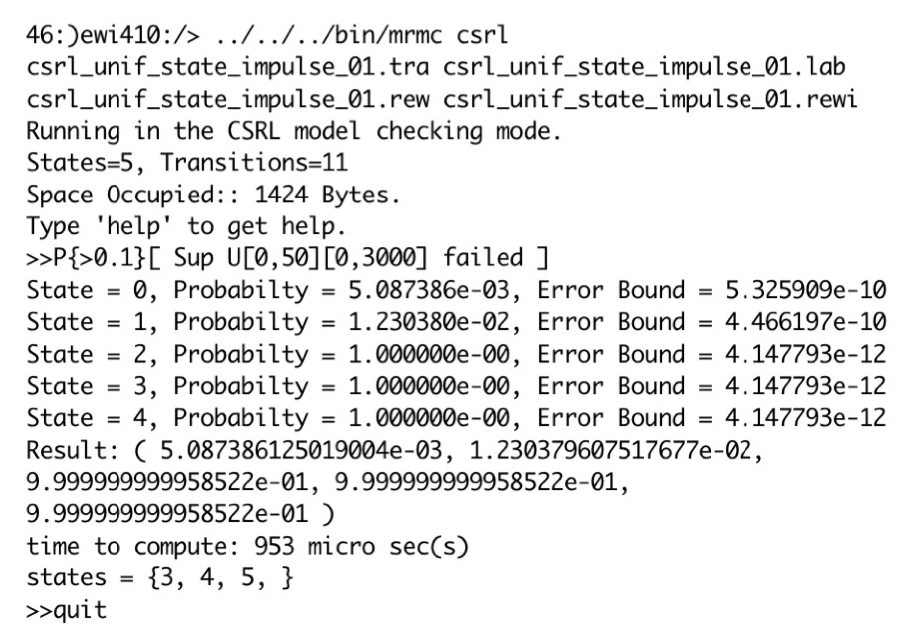
\includegraphics[scale=0.3]{qest_05_figure_02_1.eps}}
					\end{center}
				\end{example}
	       	\end{minipage} 
	       }
       	\hfill
	       \begin{minipage}[t]{0.47\linewidth}
			\begin{center}
				%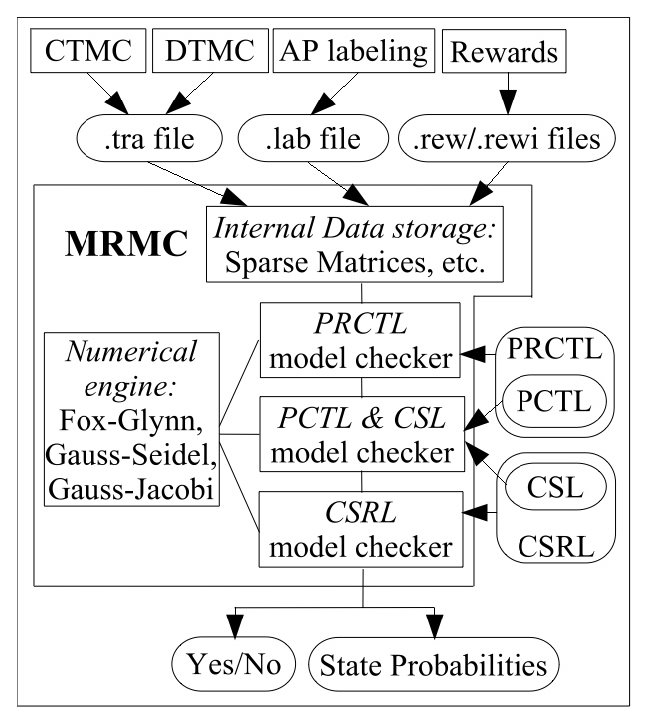
\includegraphics[scale=0.55, angle=0]{qest_05_figure_01.eps}
				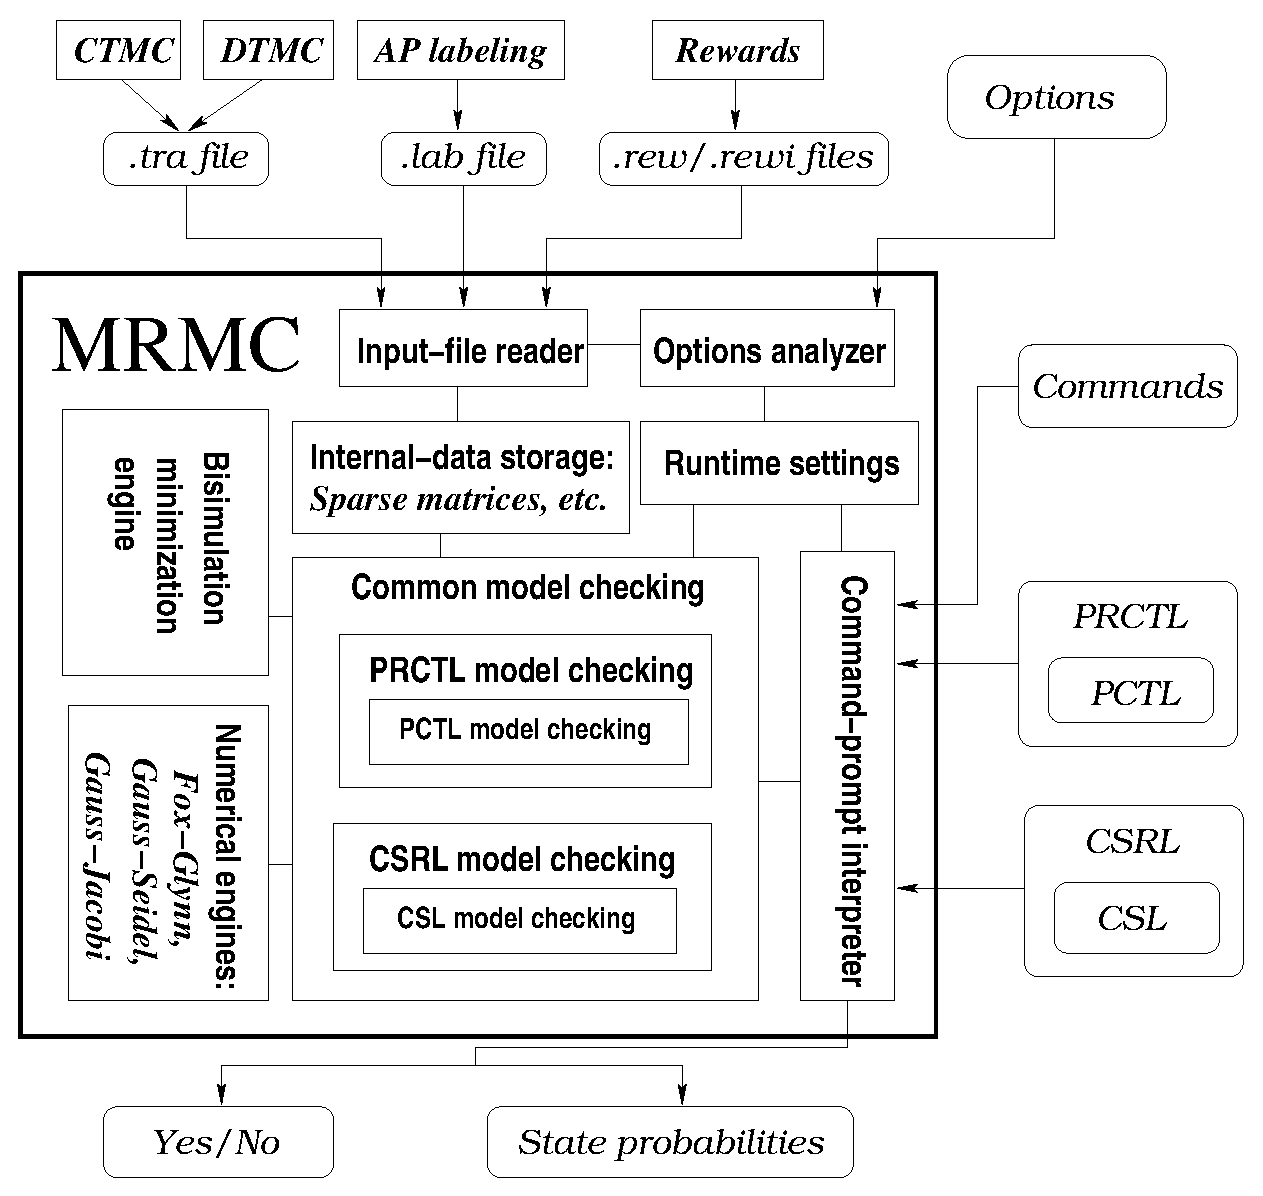
\includegraphics[scale=0.29, angle=0]{mrmc_architecture.eps}
			\end{center}
       	\end{minipage}
	}
	
	\only<2>{
		\begin{center}
			\hyperlink{cmdline<1>}{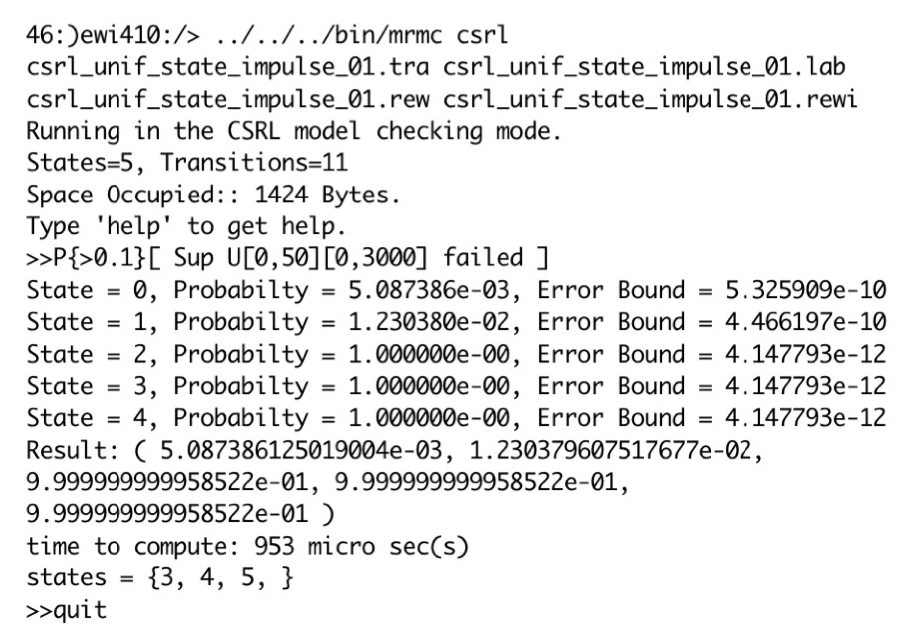
\includegraphics[scale=0.7]{qest_05_figure_02_1.eps}}
		\end{center}
	}
}

\frame{
	\frametitle{CSL logic: $\pUp{0}{t}$}
	
		\begin{center}
			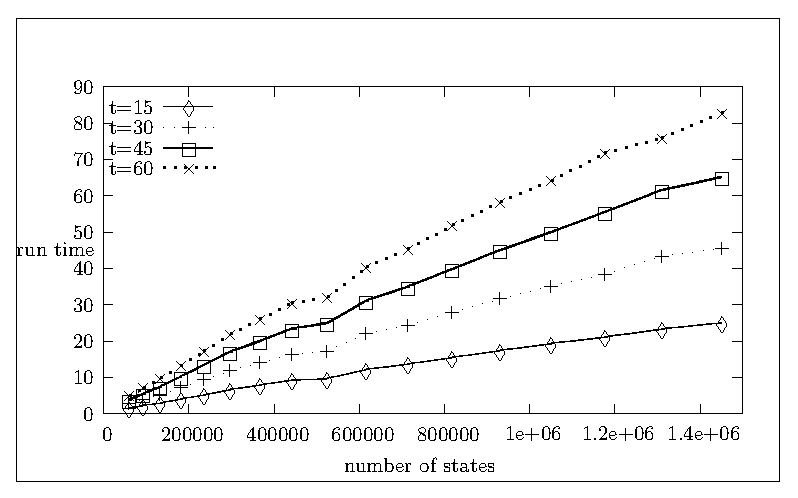
\includegraphics[scale=0.75]{qest_05_figure_03.eps}
		\end{center}
}

\frame{
	\frametitle{CSRL logic: $\pUrp{0}{t}{0}{r}$}
	
		\begin{center}
			\scalebox{0.9}[0.9]{% GNUPLOT: LaTeX picture
\setlength{\unitlength}{0.240900pt}
\ifx\plotpoint\undefined\newsavebox{\plotpoint}\fi
\sbox{\plotpoint}{\rule[-0.200pt]{0.400pt}{0.400pt}}%
\begin{picture}(1500,900)(0,0)
\font\gnuplot=cmr10 at 10pt
\gnuplot
\sbox{\plotpoint}{\rule[-0.200pt]{0.400pt}{0.400pt}}%
\put(201.0,123.0){\rule[-0.200pt]{4.818pt}{0.400pt}}
\put(181,123){\makebox(0,0)[r]{ 0}}
\put(1419.0,123.0){\rule[-0.200pt]{4.818pt}{0.400pt}}
\put(201.0,200.0){\rule[-0.200pt]{4.818pt}{0.400pt}}
\put(181,200){\makebox(0,0)[r]{ 500}}
\put(1419.0,200.0){\rule[-0.200pt]{4.818pt}{0.400pt}}
\put(201.0,277.0){\rule[-0.200pt]{4.818pt}{0.400pt}}
\put(181,277){\makebox(0,0)[r]{ 1000}}
\put(1419.0,277.0){\rule[-0.200pt]{4.818pt}{0.400pt}}
\put(201.0,354.0){\rule[-0.200pt]{4.818pt}{0.400pt}}
\put(181,354){\makebox(0,0)[r]{ 1500}}
\put(1419.0,354.0){\rule[-0.200pt]{4.818pt}{0.400pt}}
\put(201.0,431.0){\rule[-0.200pt]{4.818pt}{0.400pt}}
\put(181,431){\makebox(0,0)[r]{ 2000}}
\put(1419.0,431.0){\rule[-0.200pt]{4.818pt}{0.400pt}}
\put(201.0,508.0){\rule[-0.200pt]{4.818pt}{0.400pt}}
\put(181,508){\makebox(0,0)[r]{ 2500}}
\put(1419.0,508.0){\rule[-0.200pt]{4.818pt}{0.400pt}}
\put(201.0,585.0){\rule[-0.200pt]{4.818pt}{0.400pt}}
\put(181,585){\makebox(0,0)[r]{ 3000}}
\put(1419.0,585.0){\rule[-0.200pt]{4.818pt}{0.400pt}}
\put(201.0,662.0){\rule[-0.200pt]{4.818pt}{0.400pt}}
\put(181,662){\makebox(0,0)[r]{ 3500}}
\put(1419.0,662.0){\rule[-0.200pt]{4.818pt}{0.400pt}}
\put(201.0,739.0){\rule[-0.200pt]{4.818pt}{0.400pt}}
\put(181,739){\makebox(0,0)[r]{ 4000}}
\put(1419.0,739.0){\rule[-0.200pt]{4.818pt}{0.400pt}}
\put(201.0,123.0){\rule[-0.200pt]{0.400pt}{4.818pt}}
\put(201,82){\makebox(0,0){ 0}}
\put(201.0,757.0){\rule[-0.200pt]{0.400pt}{4.818pt}}
\put(426.0,123.0){\rule[-0.200pt]{0.400pt}{4.818pt}}
\put(426,82){\makebox(0,0){ 1000}}
\put(426.0,757.0){\rule[-0.200pt]{0.400pt}{4.818pt}}
\put(651.0,123.0){\rule[-0.200pt]{0.400pt}{4.818pt}}
\put(651,82){\makebox(0,0){ 2000}}
\put(651.0,757.0){\rule[-0.200pt]{0.400pt}{4.818pt}}
\put(876.0,123.0){\rule[-0.200pt]{0.400pt}{4.818pt}}
\put(876,82){\makebox(0,0){ 3000}}
\put(876.0,757.0){\rule[-0.200pt]{0.400pt}{4.818pt}}
\put(1101.0,123.0){\rule[-0.200pt]{0.400pt}{4.818pt}}
\put(1101,82){\makebox(0,0){ 4000}}
\put(1101.0,757.0){\rule[-0.200pt]{0.400pt}{4.818pt}}
\put(1326.0,123.0){\rule[-0.200pt]{0.400pt}{4.818pt}}
\put(1326,82){\makebox(0,0){ 5000}}
\put(1326.0,757.0){\rule[-0.200pt]{0.400pt}{4.818pt}}
\put(201.0,123.0){\rule[-0.200pt]{298.234pt}{0.400pt}}
\put(1439.0,123.0){\rule[-0.200pt]{0.400pt}{157.549pt}}
\put(201.0,777.0){\rule[-0.200pt]{298.234pt}{0.400pt}}
\put(190,815){\makebox(0,0){computation time (in s)}}
\put(820,21){\makebox(0,0){state space}}
% \put(820,875){\makebox(0,0){Uniformization}}
\put(201.0,123.0){\rule[-0.200pt]{0.400pt}{157.549pt}}
\put(661,737){\makebox(0,0)[r]{error bound: {\color[rgb]{1,0,0}{\tiny $10^{-3}$}}}}
{\color[rgb]{1,0,0} \put(681.0,737.0){\rule[-0.200pt]{24.090pt}{0.400pt}}
\put(244,123){\usebox{\plotpoint}}
\put(286,122.67){\rule{6.504pt}{0.400pt}}
\multiput(286.00,122.17)(13.500,1.000){2}{\rule{3.252pt}{0.400pt}}
\put(244.0,123.0){\rule[-0.200pt]{10.118pt}{0.400pt}}
\put(548,123.67){\rule{12.286pt}{0.400pt}}
\multiput(548.00,123.17)(25.500,1.000){2}{\rule{6.143pt}{0.400pt}}
\put(313.0,124.0){\rule[-0.200pt]{56.611pt}{0.400pt}}
\put(776,124.67){\rule{16.140pt}{0.400pt}}
\multiput(776.00,124.17)(33.500,1.000){2}{\rule{8.070pt}{0.400pt}}
\put(599.0,125.0){\rule[-0.200pt]{42.639pt}{0.400pt}}
\put(1063,125.67){\rule{19.272pt}{0.400pt}}
\multiput(1063.00,125.17)(40.000,1.000){2}{\rule{9.636pt}{0.400pt}}
\put(1143,126.67){\rule{20.236pt}{0.400pt}}
\multiput(1143.00,126.17)(42.000,1.000){2}{\rule{10.118pt}{0.400pt}}
\put(1227,126.67){\rule{21.199pt}{0.400pt}}
\multiput(1227.00,127.17)(44.000,-1.000){2}{\rule{10.600pt}{0.400pt}}
\put(1315,126.67){\rule{22.163pt}{0.400pt}}
\multiput(1315.00,126.17)(46.000,1.000){2}{\rule{11.081pt}{0.400pt}}}
\iffalse
\put(244,123){\raisebox{-.8pt}{\makebox(0,0){$\Diamond$}}}
\put(263,123){\raisebox{-.8pt}{\makebox(0,0){$\Diamond$}}}
\put(286,123){\raisebox{-.8pt}{\makebox(0,0){$\Diamond$}}}
\put(313,124){\raisebox{-.8pt}{\makebox(0,0){$\Diamond$}}}
\put(343,124){\raisebox{-.8pt}{\makebox(0,0){$\Diamond$}}}
\put(377,124){\raisebox{-.8pt}{\makebox(0,0){$\Diamond$}}}
\put(414,124){\raisebox{-.8pt}{\makebox(0,0){$\Diamond$}}}
\put(455,124){\raisebox{-.8pt}{\makebox(0,0){$\Diamond$}}}
\put(499,124){\raisebox{-.8pt}{\makebox(0,0){$\Diamond$}}}
\put(548,124){\raisebox{-.8pt}{\makebox(0,0){$\Diamond$}}}
\put(599,125){\raisebox{-.8pt}{\makebox(0,0){$\Diamond$}}}
\put(655,125){\raisebox{-.8pt}{\makebox(0,0){$\Diamond$}}}
\put(714,125){\raisebox{-.8pt}{\makebox(0,0){$\Diamond$}}}
\put(776,125){\raisebox{-.8pt}{\makebox(0,0){$\Diamond$}}}
\put(843,126){\raisebox{-.8pt}{\makebox(0,0){$\Diamond$}}}
\put(912,126){\raisebox{-.8pt}{\makebox(0,0){$\Diamond$}}}
\put(986,126){\raisebox{-.8pt}{\makebox(0,0){$\Diamond$}}}
\put(1063,126){\raisebox{-.8pt}{\makebox(0,0){$\Diamond$}}}
\put(1143,127){\raisebox{-.8pt}{\makebox(0,0){$\Diamond$}}}
\put(1227,128){\raisebox{-.8pt}{\makebox(0,0){$\Diamond$}}}
\put(1315,127){\raisebox{-.8pt}{\makebox(0,0){$\Diamond$}}}
\put(1407,128){\raisebox{-.8pt}{\makebox(0,0){$\Diamond$}}}
\put(731,737){\raisebox{-.8pt}{\makebox(0,0){$\Diamond$}}}
\fi
{\color[rgb]{1,0,0} \put(843.0,126.0){\rule[-0.200pt]{52.998pt}{0.400pt}}}
\put(661,696){\makebox(0,0)[r]{\phantom{error bound:} {\tiny $10^{-4}$}}}
\multiput(681,696)(20.756,0.000){5}{\usebox{\plotpoint}}
\put(781,696){\usebox{\plotpoint}}
\put(244,125){\usebox{\plotpoint}}
\put(244.00,125.00){\usebox{\plotpoint}}
\multiput(263,126)(20.736,0.902){2}{\usebox{\plotpoint}}
\put(306.16,128.49){\usebox{\plotpoint}}
\put(326.89,129.46){\usebox{\plotpoint}}
\multiput(343,130)(20.747,0.610){2}{\usebox{\plotpoint}}
\multiput(377,131)(20.725,1.120){2}{\usebox{\plotpoint}}
\multiput(414,133)(20.731,1.011){2}{\usebox{\plotpoint}}
\multiput(455,135)(20.734,0.942){2}{\usebox{\plotpoint}}
\multiput(499,137)(20.738,0.846){2}{\usebox{\plotpoint}}
\multiput(548,139)(20.740,0.813){3}{\usebox{\plotpoint}}
\multiput(599,141)(20.703,1.479){2}{\usebox{\plotpoint}}
\multiput(655,145)(20.744,0.703){3}{\usebox{\plotpoint}}
\multiput(714,147)(20.731,1.003){3}{\usebox{\plotpoint}}
\multiput(776,150)(20.735,0.928){3}{\usebox{\plotpoint}}
\multiput(843,153)(20.736,0.902){4}{\usebox{\plotpoint}}
\multiput(912,156)(20.738,0.841){3}{\usebox{\plotpoint}}
\multiput(986,159)(20.712,1.345){4}{\usebox{\plotpoint}}
\multiput(1063,164)(20.749,0.519){4}{\usebox{\plotpoint}}
\multiput(1143,166)(20.719,1.233){4}{\usebox{\plotpoint}}
\multiput(1227,171)(20.743,0.707){4}{\usebox{\plotpoint}}
\multiput(1315,174)(20.712,1.351){5}{\usebox{\plotpoint}}
\put(1407,180){\usebox{\plotpoint}}
\put(244,125){\makebox(0,0){{\tiny $+$}}}
\put(263,126){\makebox(0,0){{\tiny $+$}}}
\put(286,127){\makebox(0,0){{\tiny $+$}}}
\put(313,129){\makebox(0,0){{\tiny $+$}}}
\put(343,130){\makebox(0,0){{\tiny $+$}}}
\put(377,131){\makebox(0,0){{\tiny $+$}}}
\put(414,133){\makebox(0,0){{\tiny $+$}}}
\put(455,135){\makebox(0,0){{\tiny $+$}}}
\put(499,137){\makebox(0,0){{\tiny $+$}}}
\put(548,139){\makebox(0,0){{\tiny $+$}}}
\put(599,141){\makebox(0,0){{\tiny $+$}}}
\put(655,145){\makebox(0,0){{\tiny $+$}}}
\put(714,147){\makebox(0,0){{\tiny $+$}}}
\put(776,150){\makebox(0,0){{\tiny $+$}}}
\put(843,153){\makebox(0,0){{\tiny $+$}}}
\put(912,156){\makebox(0,0){{\tiny $+$}}}
\put(986,159){\makebox(0,0){{\tiny $+$}}}
\put(1063,164){\makebox(0,0){{\tiny $+$}}}
\put(1143,166){\makebox(0,0){{\tiny $+$}}}
\put(1227,171){\makebox(0,0){{\tiny $+$}}}
\put(1315,174){\makebox(0,0){{\tiny $+$}}}
\put(1407,180){\makebox(0,0){{\tiny $+$}}}
\put(731,696){\makebox(0,0){{\scriptsize $+$}}}
\sbox{\plotpoint}{\rule[-0.400pt]{0.800pt}{0.800pt}}%
\put(661,655){\makebox(0,0)[r]{\phantom{error bound:} {\color[rgb]{0,0,1} {\tiny $10^{-5}$}}}}
{\color[rgb]{0,0,1} \put(681.0,655.0){\rule[-0.400pt]{24.090pt}{0.800pt}}
\put(244,145){\usebox{\plotpoint}}
\multiput(244.00,146.40)(1.285,0.520){9}{\rule{2.100pt}{0.125pt}}
\multiput(244.00,143.34)(14.641,8.000){2}{\rule{1.050pt}{0.800pt}}
\multiput(263.00,154.41)(0.988,0.511){17}{\rule{1.733pt}{0.123pt}}
\multiput(263.00,151.34)(19.402,12.000){2}{\rule{0.867pt}{0.800pt}}
\multiput(286.00,166.41)(0.757,0.506){29}{\rule{1.400pt}{0.122pt}}
\multiput(286.00,163.34)(24.094,18.000){2}{\rule{0.700pt}{0.800pt}}
\multiput(313.00,184.40)(2.490,0.526){7}{\rule{3.629pt}{0.127pt}}
\multiput(313.00,181.34)(22.469,7.000){2}{\rule{1.814pt}{0.800pt}}
\multiput(343.00,191.41)(1.166,0.508){23}{\rule{2.013pt}{0.122pt}}
\multiput(343.00,188.34)(29.821,15.000){2}{\rule{1.007pt}{0.800pt}}
\multiput(377.00,206.41)(1.113,0.507){27}{\rule{1.941pt}{0.122pt}}
\multiput(377.00,203.34)(32.971,17.000){2}{\rule{0.971pt}{0.800pt}}
\multiput(414.00,223.41)(1.237,0.507){27}{\rule{2.129pt}{0.122pt}}
\multiput(414.00,220.34)(36.580,17.000){2}{\rule{1.065pt}{0.800pt}}
\multiput(455.00,240.41)(1.065,0.505){35}{\rule{1.876pt}{0.122pt}}
\multiput(455.00,237.34)(40.106,21.000){2}{\rule{0.938pt}{0.800pt}}
\multiput(499.00,261.41)(1.133,0.505){37}{\rule{1.982pt}{0.122pt}}
\multiput(499.00,258.34)(44.887,22.000){2}{\rule{0.991pt}{0.800pt}}
\multiput(548.00,283.41)(1.303,0.505){33}{\rule{2.240pt}{0.122pt}}
\multiput(548.00,280.34)(46.351,20.000){2}{\rule{1.120pt}{0.800pt}}
\multiput(600.41,302.00)(0.502,0.598){105}{\rule{0.121pt}{1.157pt}}
\multiput(597.34,302.00)(56.000,64.598){2}{\rule{0.800pt}{0.579pt}}
\multiput(655.00,367.08)(3.215,-0.514){13}{\rule{4.920pt}{0.124pt}}
\multiput(655.00,367.34)(48.788,-10.000){2}{\rule{2.460pt}{0.800pt}}
\multiput(714.00,360.41)(1.164,0.504){47}{\rule{2.037pt}{0.121pt}}
\multiput(714.00,357.34)(57.772,27.000){2}{\rule{1.019pt}{0.800pt}}
\multiput(776.00,387.41)(0.864,0.503){71}{\rule{1.574pt}{0.121pt}}
\multiput(776.00,384.34)(63.732,39.000){2}{\rule{0.787pt}{0.800pt}}
\multiput(843.00,426.41)(1.405,0.504){43}{\rule{2.408pt}{0.121pt}}
\multiput(843.00,423.34)(64.002,25.000){2}{\rule{1.204pt}{0.800pt}}
\multiput(912.00,451.41)(1.294,0.504){51}{\rule{2.241pt}{0.121pt}}
\multiput(912.00,448.34)(69.348,29.000){2}{\rule{1.121pt}{0.800pt}}
\multiput(986.00,480.41)(0.557,0.501){131}{\rule{1.093pt}{0.121pt}}
\multiput(986.00,477.34)(74.732,69.000){2}{\rule{0.546pt}{0.800pt}}
\put(1063,546.84){\rule{19.272pt}{0.800pt}}
\multiput(1063.00,546.34)(40.000,1.000){2}{\rule{9.636pt}{0.800pt}}
\multiput(1143.00,550.41)(1.115,0.503){69}{\rule{1.968pt}{0.121pt}}
\multiput(1143.00,547.34)(79.914,38.000){2}{\rule{0.984pt}{0.800pt}}
\multiput(1227.00,588.41)(0.556,0.501){151}{\rule{1.091pt}{0.121pt}}
\multiput(1227.00,585.34)(85.735,79.000){2}{\rule{0.546pt}{0.800pt}}
\multiput(1315.00,667.41)(0.622,0.501){141}{\rule{1.195pt}{0.121pt}}
\multiput(1315.00,664.34)(89.521,74.000){2}{\rule{0.597pt}{0.800pt}}}
\iffalse
\put(244,145){\raisebox{-.8pt}{\makebox(0,0){$\Box$}}}
\put(263,153){\raisebox{-.8pt}{\makebox(0,0){$\Box$}}}
\put(286,165){\raisebox{-.8pt}{\makebox(0,0){$\Box$}}}
\put(313,183){\raisebox{-.8pt}{\makebox(0,0){$\Box$}}}
\put(343,190){\raisebox{-.8pt}{\makebox(0,0){$\Box$}}}
\put(377,205){\raisebox{-.8pt}{\makebox(0,0){$\Box$}}}
\put(414,222){\raisebox{-.8pt}{\makebox(0,0){$\Box$}}}
\put(455,239){\raisebox{-.8pt}{\makebox(0,0){$\Box$}}}
\put(499,260){\raisebox{-.8pt}{\makebox(0,0){$\Box$}}}
\put(548,282){\raisebox{-.8pt}{\makebox(0,0){$\Box$}}}
\put(599,302){\raisebox{-.8pt}{\makebox(0,0){$\Box$}}}
\put(655,369){\raisebox{-.8pt}{\makebox(0,0){$\Box$}}}
\put(714,359){\raisebox{-.8pt}{\makebox(0,0){$\Box$}}}
\put(776,386){\raisebox{-.8pt}{\makebox(0,0){$\Box$}}}
\put(843,425){\raisebox{-.8pt}{\makebox(0,0){$\Box$}}}
\put(912,450){\raisebox{-.8pt}{\makebox(0,0){$\Box$}}}
\put(986,479){\raisebox{-.8pt}{\makebox(0,0){$\Box$}}}
\put(1063,548){\raisebox{-.8pt}{\makebox(0,0){$\Box$}}}
\put(1143,549){\raisebox{-.8pt}{\makebox(0,0){$\Box$}}}
\put(1227,587){\raisebox{-.8pt}{\makebox(0,0){$\Box$}}}
\put(1315,666){\raisebox{-.8pt}{\makebox(0,0){$\Box$}}}
\put(1407,740){\raisebox{-.8pt}{\makebox(0,0){$\Box$}}}
\put(731,655){\raisebox{-.8pt}{\makebox(0,0){$\Box$}}}
\fi
\end{picture}
}
		\end{center}
}

{\tiny \bibliography{../../../../BibTex/global_etmcc}}

%APPENDIX
\appendix

\AtBeginSubsection{}

\section{\appendixname}

\againframe<beamer| beamer:2>{rewex}

\againframe<beamer| beamer:2>{cmdline}

\end{document}
 